\begin{dang}{Tìm Max-min của hàm số cho bởi công thức}
    Tìm giá trị lớn nhất và giá trị nhỏ nhất của hàm số $y=f(x)$ trên đoạn $\left[a;b\right]$.
    \begin{itemize}
        \item \textbf{Bước 1.} Hàm số đã cho xác định và liên tục trên đoạn $\left[a;b\right]$.\\
        Tính $f'(x)$ và tìm những điểm $x_i$ sao cho tại đó có đạo hàm bằng $0$ hoặc liên tục nhưng không có đạo hàm.
        \item \textbf{Bước 2.} Tính $f(a)$, $f(b)$, $f(x_i)$.
        \item \textbf{Bước 3.} Kết luận$\colon \heva{&\max\limits_{[a;b]} f(x)=\max\{f(a); f(b); f(x_i)\}\\ &\min\limits_{[a;b]} f(x)=\min\{f(a); f(b); f(x_i)\}.}$
    \end{itemize}
    \begin{nx}
        \begin{itemize}
            \item Nếu hàm số $y=f(x)$ đồng biến trên $[a;b]$ thì $\min \limits_{[a;b]} f(x)=f(a)$ và $\max \limits_{[a;b]} f(x)= f(b)$.
            \item Nếu hàm số $y=f(x)$ nghịch biến trên $[a;b]$ thì $\max \limits_{[a;b]} f(x)=f(a)$ và $\min \limits_{[a;b]} f(x)= f(b)$.
            \item Nếu tìm GTLN và GTNN của hàm số $y=f(x)$ không phải trên $[a;b]$ thì lập bảng biến thiên để kết luận.
        \end{itemize}
    \end{nx}
\end{dang}
\begin{vd}
    Tìm Max-min của hàm số
    \begin{listEX}[3]
        \item $y=x^3-24x$ trên $[2;19]$.
        \item $y=\dfrac{3x-1}{x-3}$ trên $[0;2]$.
        \item $y=x+\dfrac{9}{x}$ trên $[2;4]$.
        \item $y=\sqrt{9-x^2}$
        \item $y=\dfrac{\ln x}{x}$
        \item $y=\sin^5x-2\sin^3x+2$
        % \item $y=|x^3-3x+1|$ trên $[0;3]$
    \end{listEX}
    \loigiai{}
\end{vd}
\begin{vd}
    Tìm $m$ để hàm số
    \begin{listEX}
        \item $y=x^3-3x^2-9x+m$ có giá trị lớn nhất trên $[1;4]$ bằng $5$.
        \item $y=\dfrac{mx+1}{x-1}$ có giá trị nhỏ nhất trên $[-1;2]$ bằng 3.
    \end{listEX}
    \loigiai{}
\end{vd}
\BTTN
\Opensolutionfile{ans}[ans/2D1-3-DANG-2]
\begin{ex}%[HK1, Sở GD và ĐT - Đà Nẵng, 2020-2021]%[Lê Vũ Hải, 12EX4]%[2D1Y3-1]%
    Giá trị lớn nhất của hàm số $y=x^3-3x+1$ trên đoạn $[-2;2]$ là
    \choice
    {$-1$}
    {$2$}
    {\True $3$}
    {$-2$}
    \loigiai{
        Ta có $y'=3x^2-3 \Rightarrow y'=0 \Leftrightarrow \hoac{&x=1 \\ &x=-1.}$\\
        Ta có $y(-2)=-1$, $y(2)=3$, $y(1)=-1$, $y(-1)=3$.\\
        Vậy $\max\limits_{[-2;2]} y = 3$.
    }
\end{ex}
\begin{ex}%[2D1Y3-1]%
    Tìm giá trị nhỏ nhất của hàm số $y=\dfrac{1}{4}x^4-2x^2+\dfrac{5}{4}$ trên đoạn $[0;3]$.
    \choice
    {$\dfrac{9}{2}$}
    {$\dfrac{7}{2}$}
    {$1$}
    {\True $-\dfrac{11}{4}$}
    \loigiai
    {
        Hàm số đã cho xác định và liên tục trên $ [0; 3] $.\\
        Ta có $y'=x^3-4x$, $ y'=0\Leftrightarrow x^3-4x=0\Leftrightarrow\hoac{&x=0\in[0; 3]\\&x=2\in[0; 3]\\&x=-2\notin[0;3].} $\\
        Mà $y(0)=\dfrac{5}{4};~y(2)=-\dfrac{11}{4};~y(3)=\dfrac{7}{2}$.\\
        Suy ra $\min\limits_{[0;3]}y=-\dfrac{11}{4}$.
    }
\end{ex}
\begin{ex}%[2D1Y3-1]%
    Giá trị lớn nhất và giá trị nhỏ nhất của hàm số $y=x^4-2x^2+3$ trên $[0;2]$ lần lượt là $M$ và $m$. Khẳng định nào sau đây đúng?
    \choice
    {$M=5,m=2$}
    {$M=3,m=2$}
    {\True $M=11,m=2$}
    {$M=11,m=3$}
    \loigiai{
        Hàm số đã cho xác định và liên tục trên $ [0; 2] $.\\
        Ta có $y'=4x^3-4x;\,y'=0\Leftrightarrow\hoac{&x=0\in[0;2]\\&x=1\in[0;2]\\&x=-1\notin [0;2].}$\\
        Mà $f(0)=3$, $f(1)=2$, $f(2)=11$.\\
        Vậy $M=11$, $m=2$.
    }
\end{ex}
\begin{ex}%[Đề thi giữa HK1, THPT Bình Sơn Đồng Nai, 2019]%[Phan Minh Tâm, dự án EX3]%[2D1Y3-1]%
    Giá trị lớn nhất của hàm số $ y = \sqrt{1-x^2} $ bằng
    \choice
    {\True $ 1 $}
    {$ 0$}
    {$ -1 $}
    {$ 2 $}
    \loigiai
    { 	Ta có $ y = \sqrt{1-x^2} \le 1, \forall x \in \left[-1;1\right]$.\\ Do vậy giá trị lớn nhất của hàm số $ y = \sqrt{1-x^2} $ là $ 1 $ tại $ x=0 $.
    }
\end{ex}
\begin{ex}%[2D1Y3-1]%
    Giá trị nhỏ nhất của hàm số $y=2x^3+3x^2-12x+2$ trên đoạn $[-1;2]$ đạt tại $x=x_0$. Giá trị $x_0$ bằng bao nhiêu?
    \choice
    {$2$}
    {\True $1$}
    {$-2$}
    {$-1$}
    \loigiai{
        Xét hàm số $y=2x^3+3x^2-12x+2$ trên đoạn $[-1;2]$, ta có $y'=6x^2+6x-12 = 0 $ có nghiệm $x=1 \in (-1;2)$. Vì $f(-1)=15$, $f(2)=6$, $f(1)=-5$ nên ta có $x_0=1$.
    }
\end{ex}
\begin{ex}%[GHK1, THPT Trần Hưng Đạo - Nam Định, 2019]%[Đặng Tân Hoài, 12-EX-3-2019]%[2D1Y3-1]%
    Gọi $m$ là giá trị nhỏ nhất của hàm số $y=\dfrac{3x+1}{x-2}$ trên $[-1;1]$. Khi đó giá trị của $m$ là
    \choice
    {$ m=\dfrac{2}{3} $}
    {$ m=-\dfrac{2}{3} $}
    {\True $ m=-4 $}
    {$ m=4 $}
    \loigiai{
        Vì hàm số $y=\dfrac{ax+b}{cx+d}$ luôn đơn điệu trên một đoạn không chứa $x=-\dfrac{d}{c}$ nên hàm số đạt GTLN, GTNN tại các điểm đầu mút của đoạn đó.\\
        Ta có $y'=\dfrac{-7}{(x-2)^2}<0, ~ \forall x \neq 2$.
        Do đó $\min\limits_{[-1;1]} y = y(1)=\dfrac{3\cdot1+1}{1-2}=-4$.
    }
\end{ex}
\begin{ex}%[THPTQG 2020 câu 26 đề 102]%[2D1B3-1]
    Giá trị nhỏ nhất của hàm số $f(x)=x^3-21x$ trên đoạn $[2;19]$ bằng
    \choice
    {$-36$}
    {\True$-14\sqrt{7}$}
    {$14\sqrt{7}$}
    {$-34$}
    \loigiai{
        Ta có $f'(x)=3x^2-21=3(x^2-7)$ nên $f'(x)=0\Leftrightarrow x=\sqrt{7}$ vì $x\in[2;19]$.\\
        Ta có bảng biến thiên
        \begin{center}
            \begin{tikzpicture}
                \tkzTabInit[nocadre=false,lgt=1.2,espcl=2.5,deltacl=0.6]
                {$x$/.6,$f'(x)$/.6,$f(x)$/2}
                {$2$,$\sqrt{7}$,$19$}
                \tkzTabLine{ , - , $0$ , + , }
                \tkzTabVar{+/$-34$ , -/$-14\sqrt{7}$, +/$6403$}
            \end{tikzpicture}
        \end{center}
        Vậy $\min\limits_{[2;19]} f(x)=-14\sqrt{7}$.
    }
\end{ex}
\begin{ex}%[Nguyễn Thế Út - DA1]%[2D1B3-1]
    Giá trị lớn nhất của hàm số $f(x)=x^4-2x^2+3$ trên đoạn $\left[ 0;\sqrt{3}\right] $ bằng
    \choice
    {$9$}
    {$8\sqrt{3}$}
    {\True $6$}
    {$1$}
    \loigiai{
        Hàm số liên tục trên $\left[ 0;\sqrt{3}\right] $.\\
        Ta có $f'(x)=4x^3-4x=4x(x^2-1)$. $$f'(x)=0\Leftrightarrow4x(x^2-1)=0\Leftrightarrow \hoac{& x=0\in [0;\sqrt{3}] \\ & x=1\in [0;\sqrt{3}]\\& x=-1\notin[0;\sqrt{3}].}$$
        Mà $f(0)=3$, $f(1)=2$, $f(\sqrt{3})=6$.\\
        Vậy $\max\limits_{x \in [0;\sqrt{3}]} f(x)=6$.
    }
\end{ex}
\begin{ex}%[Nguyễn Thế Út - DA1]%[2D1B3-1]
    Tổng giá trị lớn nhất và giá trị nhỏ nhất của hàm số $f(x)=x^5-5x^4+5x^3+1$ trên đoạn $[-1;2]$ bằng
    \choice
    {$-4$}
    {$8$}
    {$4$}
    {\True $-8$}
    \loigiai{
        Hàm số liên tục trên $[-1;2]$.\\
        Ta có $f'(x)=5x^4-20x^3+15x^2$. $$f'(x)=0\Leftrightarrow 5x^4-20x^3+15x^2=0 \Leftrightarrow\hoac{& x=0\in [-1;2] \\ & x=1\in[-1;2]\\& x=3\notin[-1;2].}$$
        Ta có $f(-1)=-10, f(0)=1, f(1)=2, f(2)=-7$.\\
        Suy ra $\max\limits_{x \in [-1;2]} f(x)=2$ và $ \min\limits_{x \in [-1;2]} f(x)=-10 $.\\
        Vậy tổng giá trị lớn nhất và giá trị nhỏ nhất là $ -8 $.
    }
\end{ex}
\begin{ex}%[Dự án tex hóa đề cương Mariecurie - Biên soạn Thầy Nguyễn Ngọc Nguyên]%[2D1Y3-1]
    Gọi $M$ và $m$ lần lượt là giá trị lớn nhất và giá trị nhỏ nhất của hàm số \break $f(x)=x^3+3x^2-9x-7$ trên đoạn $[-4;3]$. Giá rị $M-m$ bằng
    \choice
    {$33$}
    {$25$}
    {\True $32$}
    {$8$}
    \loigiai{
        Ta có $y'=3x^2+6x-9$. Giải $y'=0 \Leftrightarrow \hoac{& x=1 \in [-4;3] \\ & x=-3 \in [-4;3].}$\\
        Tính $f(-4)=13$, $f(-3)=20$, $f(1)=-12$, $f(3)=20$.\\
        Ta có $M=\max \limits_{[-4;3]} f(x)= 20$, $m=\min \limits_{[-4;3]} f(x)= -12$.\\
        Ta có $M-m=20-(-12)=32$.
    }
\end{ex}
\begin{ex}%[2D1Y3-1]%
    Tìm giá trị nhỏ nhất $m$ của hàm số $y = x^3 - 7x^2 + 11x - 2$ trên đoạn $\left[0; 2\right]$.
    \choice
    {\True $m = - 2$}
    {$m = 11$}
    {$m = 0$}
    {$m = 3$}
    \loigiai{
        Hàm số đã cho xác định và liên tục trên đoạn $ [0; 2] $.\\
        Ta có $y' = 3x^2 - 14x + 11 \Rightarrow y' = 0 \Leftrightarrow 3x^2 - 14x + 11 = 0 \Leftrightarrow \hoac{&x = 1\in[0; 2]\\&x = \dfrac{11}{3}\notin[0; 2].}$\\
        Khi đó $y\left(0\right) = -2, y\left(1\right) = 3$ và $y\left(2\right) = 0 \Rightarrow \min\limits_{x \in \left[0;2\right]} y = y\left(0\right) = - 2$.
    }
\end{ex}
\begin{ex}%[Thi thử L2, Chuyên Lê Quý Đôn Quảng Trị, 2018]%[Đậu Anh Hùng, dự án EX10]%[2D1Y3-1]%
    Giá trị nhỏ nhất của hàm số $y=\dfrac{2x+1}{1-x}$ trên đoạn $[2;3]$ bằng
    \choice
    {$\dfrac{3}{4}$}
    {\True $-5$}
    {$-\dfrac{7}{2}$}
    {$-3$}
    \loigiai{Ta có $y'=\dfrac{3}{(1-x)^2}>0,\, \forall x\ne 1$, suy ra hàm số đồng biến trên $[2;3]$. Do đó, giá trị nhỏ nhất của hàm số trên $[2;3]$ là $f(2)=-5$.}
\end{ex}
\begin{ex}%[2D1Y3-1]%Câu 18
    Giá trị lớn nhất của hàm số $y=x^3-3x+5$ trên đoạn $\left[0;\dfrac{3}{2}\right]$ là:
    \choice
    {$3$}
    {\True $5$}
    {$7$}
    {$\dfrac{31}{8}$}
    \loigiai{Ta có: $y'=3x^2-3$.\\
        $y'=0 \Leftrightarrow \hoac{&x=1& \in \left[0;\dfrac{3}{2}\right]\\&x=-1&\notin \left[0;\dfrac{3}{2}\right]}$\\
        $y(0)=5,\, y(1)=3,\, y\left(\dfrac{3}{2}\right)=\dfrac{31}{8}$.\\
        Vậy giá trị lớn nhất của hàm số $y=x^3-3x+5$ trên đoạn $\left[0;\dfrac{3}{2}\right]$ bằng $5$.
    }
\end{ex}
\begin{ex}%[Dự án DeKiemtradinhki-Lan 1]%[Đoàn Minh Tân-Phản biện: Ngụy Như Thái]%[2D1Y3-1]%
    Giá trị lớn nhất của hàm số $f(x)=x^4-2x^2+1$ trên $[0;2]$ là
    \choice
    {$\max \limits_{[0;2]} f(x)=0$}
    {$\max \limits_{[0;2]} f(x)=1$}
    {$\max \limits_{[0;2]} f(x)=64$}
    {\True $\max \limits_{[0;2]} f(x)=9$}
    \loigiai{
        Ta có $f'(x)=4x^3-4x$, $4x^3-4x=0 \Rightarrow x=1 \in [0;2]$.\\
        Lại có $f(0)=1$; $f(1)=0$; $f(2)=9$.\\
        Do đó $\max \limits_{[0;2]} f(x)=9$ khi $x=2$.}
\end{ex}
\begin{ex}%[2D1B3-1]%[DeHKI-12]%[Vô Văn Tự]%7
    Giá trị nhỏ nhất của hàm số $f(x)=-x^4+4x^2-5$ trên đoạn $[-2;3]$ bằng
    \choice
    {\True $-50$}
    {$-1$}
    {$-197$}
    {$-5$}
    \loigiai{
        Tập xác định $\mathscr{D}=\mathbb{R}$.\\
        Hàm số liên tục trên $\mathbb{R}$ nên cũng liên tục trên đoạn $[-2;3]$.\\
        $y'=-4x^3+8x$; $y'=0\Leftrightarrow\hoac{&x=0\\&x=\pm\sqrt{2}.}$\\
        $y(-2)=-5$; $y(0)=-5$; $y(\pm\sqrt{2})=-1$; $y(3)=-50$.\\
        Vậy $\displaystyle\min_{[-2;3]}y=y(3)=-50$.
    }
\end{ex}
\begin{ex}%[HK1, THPT Xuân Hòa, Vĩnh Phúc, 2018]%[Đức Nguyễn,12EX-5]%[2D1B3-1]%
    Cho hàm số $y=\sqrt{-x^2+2x}$. Giá trị lớn nhất của hàm số đã cho bằng
    \choice
    {$0$}
    {\True $1$}
    {$2$}
    {$\sqrt{3}$}
    \loigiai{ Hàm số xác định khi $-x^2+2x\geq 0\Leftrightarrow 0\leq x\leq 2$.\\
        Khi đó, ta có $y=\sqrt{-x^2+2x}=\sqrt{1-\left(x-1\right)^2}\leq 1,\forall x\in \left[0;2\right]$; $y=1\Leftrightarrow \hoac{&x=2\\&x=0.}$\\
        Vậy giá trị lớn nhất của hàm số đã cho bằng $1$.
    }
\end{ex}
\begin{ex}%[Thi thử tốt nghiệp, Sở GD-ĐT Thái Nguyên, Lần 1, 2021]%[Đoàn Minh Tân, 12EX6]%[2D1B3-1]%
    Gọi $M$, $m$ lần lượt là giá trị lớn nhất, giá trị nhỏ nhất của hàm số $f(x)=x+\sqrt{4-x^2}$. Giá trị của $M-m$ bằng
    \choice
    {$4$}
    {$2\sqrt{2}-2$}
    {\True $2+2\sqrt{2}$}
    {$2\sqrt{2}$}
    \loigiai{
        Tập xác định $\mathscr{D}=[-2;2]$.\\
        $f'(x)=1-\dfrac{x}{\sqrt{4-x^2}}=\dfrac{\sqrt{4-x^2}-x}{\sqrt{4-x^2}}$.\\
        $f'(x)=0\Leftrightarrow \sqrt{4-x^2}=x\Leftrightarrow \heva{& x\ge 0\\ & 4-x^2=x^2}\Leftrightarrow \heva{& x\ge 0\\ &x=\pm \sqrt{2}}\Leftrightarrow x=\sqrt{2}$.\\
        Bảng biến thiên
        \begin{center}
            \begin{tikzpicture}
                \tkzTabInit[nocadre=false,lgt=1,espcl=3,deltacl=.6]
                {$x$/0.6,$y'$/0.6,$y$/2}
                {$-2$,$\sqrt{2}$,$+2$}
                \tkzTabLine{,+,0,-}
                \tkzTabVar{-/$-2$,+/$2\sqrt{2}$,-/$2$}
            \end{tikzpicture}
        \end{center}
        Từ bảng biến thiên, suy ra $M=\displaystyle \max\limits_{\mathscr{D}}f(x)=2\sqrt{2}$, $m=\displaystyle \min\limits_{\mathscr{D}}f(x)=-2$.\\
        Vậy $M-m=2\sqrt{2}+2$.
    }
\end{ex}
\begin{ex}%[Nguyễn Thế Út - DA1]%[2D1B3-1]
    Giá trị nhỏ nhất của hàm số $f(x)=\dfrac{-2x+3}{x+1}$ trên đoạn $[1;4]$ bằng.
    \choice
    {$1$}
    {\True $-1$}
    {$\dfrac{1}{2}$}
    {$-\dfrac{1}{2}$}
    \loigiai{
        \begin{itemize}
            \item Tập xác định $\mathscr{D}=\mathbb{R}\setminus\{-1\}$.
            \item Ta có $f'(x)=-\dfrac{-5}{(x+1)^2}<0$, $\forall x\in\mathscr{D}$.
            \item Do đó hàm số nghịch biến trên $[1;4]$. Suy ra $\min\limits_{[1;4]}f(x)=f(4)=-1$.
        \end{itemize}
    }
\end{ex}
\begin{ex}%[Nguyễn Thế Út - DA1]%[2D1B3-1]
    Giá trị lớn nhất của hàm số $f(x)=\dfrac{3x-1}{x-3}$ trên đoạn $[0;2]$ bằng.
    \choice
    {$5$}
    {$-5$}
    {\True $\dfrac{1}{3}$}
    {$-\dfrac{1}{3}$}
    \loigiai{
        \begin{itemize}
            \item Tập xác định $\mathscr{D}=\mathbb{R}\setminus\{3\}$.
            \item Ta có $f'(x)=-\dfrac{8}{(x-3)^2}<0$, $\forall x\in\mathscr{D}$.
            \item Do đó hàm số nghịch biến trên $[0;2]$. Suy ra $\max\limits_{[0;2]}f(x)=f(0)=\dfrac{1}{3}$.
        \end{itemize}
    }
\end{ex}
\begin{ex}%[Nguyễn Thế Út - DA1]%[2D1B3-1]
    Giá trị lớn nhất của hàm số $y=x+\dfrac{1}{x}$ trên đoạn $[1;3]$ bằng
    \choice
    {$2$}
    {$\dfrac{11}{3}$}
    {$\dfrac{12}{5}$}
    {\True $\dfrac{10}{3}$}
    \loigiai{
        Ta có $y'=1-\dfrac{1}{x^2}$.
        $$y'=0\Leftrightarrow \hoac{&x=1\in [1;3]\\&x=-1\notin[1;3].}$$
        Khi đó $f(1)=2,f(3)=\dfrac{10}{3}$, suy ra $\max\limits_{[1;3]}f(x)=\dfrac{10}{3}$.
    }
\end{ex}
\begin{ex}%[Nguyễn Trần Phong, Dự án 6 đề cương HKI k12 Marie]%[2D1B3-1]
    Giá trị nhỏ nhất của hàm số $y= \dfrac{x^2 -3x+1}{x+1}$ trên đoạn $[1;4]$ bằng
    \choice
    {$ - \dfrac{1}{2}$}
    {\True $-5 + 2 \sqrt{5} $}
    {$-5 - 2 \sqrt{5} $}
    {$ 1$}
    \loigiai{
        Ta có $y'= \dfrac{x^2 + 2x -4 }{(x+1)^2}$.\\
        Cho $y'=0 \Leftrightarrow x^2 + 2x -5 =0 \Leftrightarrow \hoac{&x = -1 + \sqrt{5} \in [1;4] \\& x= -1- \sqrt{5} \notin [1;4].}$\\
        Mà $y(1)= - \dfrac{1}{2}$; $y(4)= 1$; $y \left(-1 + \sqrt{5} \right)= -5 + 2 \sqrt{5}.$\\
        Do đó, giá trị nhỏ nhất của hàm số trên đoạn $[1;4]$ bằng $-5 + 2 \sqrt{5}$ tại $x = -1 + \sqrt{5}.$}
\end{ex}
\begin{ex}%[Nguyễn Trần Phong, Dự án 6 đề cương HKI k12 Marie]%[2D1B3-1]
    Gọi $M$, $m$ lần lượt là giá trị lớn nhất, giá trị nhỏ nhất của hàm số $y=x-5 + \dfrac{1}{x}$ trên đoạn $\left[\dfrac{1}{2};5 \right]$. Khi đó $M+ m$ bằng
    \choice
    {\True $- \dfrac{14}{5} $}
    {$- \dfrac{4}{5} $}
    {$- \dfrac{3}{4} $}
    {$- \dfrac{11}{4} $}
    \loigiai{
        Ta có $y'= 1 - \dfrac{1}{x^2}$.\\
        Cho $y'=0 \Leftrightarrow \hoac{&x=-1 \notin \left[\dfrac{1}{2};5 \right] \\& x=1 \in \left[\dfrac{1}{2};5 \right] .}$\\
        Lại có $ y \left(\dfrac{1}{2} \right) =- \dfrac{5}{2}$; $y(1)=-3$; $y(5)=\dfrac{1}{5}$.\\
        Vậy $M = \dfrac{1}{5}$; $m = -3$ và $M+ m = - \dfrac{14}{5}.$}
\end{ex}
\begin{ex}%[Nguyễn Thế Út - DA1]%[2D1B3-1]
    Cho hàm số $ y=\cos^3x +2\sin^2x+\cos x$. Giá trị lớn nhất của hàm số đã cho bằng
    \choice
    {$\dfrac{9}{4}$}
    {$-2$}
    {\True $\dfrac{58}{27}$}
    {$2$}
    \loigiai{
        Ta có $ y=\cos^3x +2\sin^2x+\cos x =\cos^3x +2(1-\cos^2x)+\cos x =\cos^3x-2\cos^2x+\cos x+2$.\\
        Đặt $ t=\cos x,\, t\in [-1;1] $. Ta được $ f(t)=t^3-2t^2 +t+2$.\\
        Ta có $ f'(t)=3t^2-4t+1;\,y'=0\Leftrightarrow \hoac{&t=1\in[-1;1]\\&t=\dfrac{1}{3}\in[-1;1].} $\\
        Mà $f\left(-1\right)=-2$, $ f\left(\dfrac{1}{3}\right)=\dfrac{58}{27} $, $f(1)=2$ nên $\max\limits_{x\in \mathbb{R}}y=\min\limits_{\left[-1;1\right]}f(t)=\dfrac{58}{27}$.}
\end{ex}
\begin{ex}%[Nguyễn Thế Út - DA1]%[2D1B3-1]
    Cho hàm số $ y=\sin^3x -\cos 2x+1$. Giá trị nhỏ nhất của hàm số đã cho bằng
    \choice
    {$\dfrac{80}{27}$}
    {\True $0$}
    {$1$}
    {$3$}
    \loigiai{
        Ta có $ y=\sin^3x -\cos 2x+1 =\sin^3x -\left(1-2\sin^2x \right) +1=\sin^3x +2\sin^2x $.\\
        Đặt $ t=\sin x,\, t\in [-1;1] $. Ta được $ f(t)=t^3+3t^2 $.\\
        Ta có $ f'(t)=3t^2+4t;\,y'=0\Leftrightarrow \hoac{&t=0\in[-1;1]\\&t=-\dfrac{4}{3}\notin[-1;1].} $\\
        Mà $f\left(-1\right)=1$, $ f\left(0\right)=0 $, $f(1)=5$ nên $\min\limits_{x\in \mathbb{R}}y=\min\limits_{\left[-1;1\right]}f(t)=0$.}
\end{ex}
%Câu 59
\begin{ex}%[2D1K3-1]%[Dự án TEX hóa đề cương Marie Curie - Ân Trương]
    \immini[thm]
    {
        Cho hàm số $ y=f(x) $ có đạo hàm liên tục trên đoạn $ [a;b] $ và $ f(1)=1 $, $ f(-1)=-\dfrac{1}{3} $. Đặt $ g(x)=f^2(x)-4f(x) $. Đồ thị của hàm số $ y=f'(x) $ là đường cong ở hình vẽ. Mệnh đề nào sau đây đúng ?
        \choice
        {\True$\min\limits_{[a;b]}g(x)=-3$}
        {$\max\limits_{[a;b]}g(x)=-3$}
        {$\min\limits_{[a;b]}g(x)=\dfrac{13}{9}$}
        {$\max\limits_{[a;b]}g(x)=\dfrac{13}{9}$}
    }
    {
        \begin{tikzpicture}[>=stealth,x=1cm,y=1cm,scale=0.8,font=\footnotesize]
            \path
            (-2.1,0) coordinate (Af)(2.1,0) coordinate (Bf)
            (0,0) coordinate (O)node[below left]{$ O $}
            (-2,2.4) coordinate (N)
            (-1.3,0) coordinate (A)
            (0.6,1) coordinate (M)node[shift={(0.6,0.2)}]{$ y=f'(x)$}
            (1.7,-1.4) coordinate (Q)
            ;
            %	\draw[red] (N)--(A2)--(M)--(Q);
            \draw[name path=ox] (Af)--(Bf);
            \draw[name path=fx,thick]
            (N)..controls +(-80:0.5) and+(170:0.5)..
            (A)..controls +(9:0.5) and+(-172:0.7)..(M)
            ..controls +(-5:0.6) and+(120:0.25)..(Q)
            ;
            \path[name intersections={of=fx and ox, by={A,B}}] ;
            %Vẽ hệ trục tọa dộ:
            \draw[->] (-2.5,0)--(0,0)--(2.5,0) node[below]{$x$};
            \draw[->] (0,-1.5) --(0,2.8) node[left]{$y$};
            %	Node các điểm
            \foreach \p in {N,A,B,Q,O}
            \fill (\p) circle (1.5pt) ;
            %	Vẽ nét đứt+node:
            \foreach \p/\n/\r in {N/a/-90,A/-1/-90,B/1/-120,Q/b/90}
            \draw[dashed](\p)--($(Af)!(\p)!(Bf)$)node[shift={(\r:3mm)}]{$ \n $} ;
        \end{tikzpicture}
    }
    \loigiai{
        Ta có bảng biến thiên của hàm số $ y=f(x) $
        \begin{center}
            \begin{tikzpicture}
                \tkzTabInit[nocadre=false,lgt=1.2,espcl=2.,deltacl=0.7]
                {$x$ /0.6,$f’(x)$ /0.6,$f(x)$ /2}
                {$a$,$-1$,$1$,$b$}
                \tkzTabLine{,+,0,-,0,-,}
                \tkzTabVar{-/ , R/ , +/$ 1 $ , -/ }
                \tkzTabIma{1}{3}{2}{$-\dfrac{1}{3}$}
            \end{tikzpicture}
        \end{center}
        Từ bảng biến thiên $ \Rightarrow f(x)\leq 1,\quad \forall x \in [a;b] $.\\
        Ta có $ g'(x)=2f(x)\cdot f'(x) -4 f'(x)=2f'(x)\cdot\left [f(x)-2\right ] $.\\
        Cho $ g'(x)=0 \Leftrightarrow\hoac{& f'(x)=0&(1) \\ & f(x)=2&(2)} $\\
        Dựa vào đồ thị, $ (1) \Leftrightarrow \hoac{& x=-1 \\ & x=1.}$\\
        Mặt khác ta có $ f(x)\leq 1, \forall x \in [a;b] \Rightarrow f(x)-2<0, \forall x \in [a;b] $.\\
        Vậy phương trình $ (2) $ vô nghiệm.\\
        Do đó, phương trình $ g'(x)=0 $ có hai nghiệm là $ x=-1 $, $ x=1 $.
        \begin{center}
            \begin{tikzpicture}
                \tkzTabInit[nocadre=false,lgt=1.2,espcl=2.,deltacl=0.7]
                {$x$ /0.6,$g’(x)$ /0.6,$g(x)$ /2.5}
                {$a$,$-1$,$1$,$b$}
                \tkzTabLine{,-,0,-,0,+,}
                \tkzTabVar{+/$ g(a) $\ , R/ , -/$ g(1) $ , +/$ g(b) $ }
            \end{tikzpicture}
        \end{center}
        Từ bảng biến thiên, suy ra
        $ \heva{& \min\limits_{[a;b]}g(x)=g(1)=f^2(1)-4f(1)=-3\\ & \max\limits_{[a;b]}g(x)=\max\left \{g(a);g(b)\right \}.} $
    }
\end{ex}
\BTTF
\begin{ex}
    Cho hàm số $f(x)=x^3-24x$. Các mệnh đề sau đúng hay sai
    \choiceTF
    {Hàm số nghịch biến trên khoảng $(-\infty ; 0)$}
    {\True Đồ thị hàm số có điểm cực tiểu là $A(16 ;-2048)$}
    {\True Giá trị lớn nhất của hàm số trên đoạn $[2 ; 19]$ bằng $6403$.}
    {Giá trị nhỏ nhất của hàm số trên đoạn $[2 ; 19]$ bằng $-40$.}
    \loigiai{Ta có $f^{\prime}(x)=3 x^2-24=0 \Leftrightarrow\left[\begin{array}{l}x=2 \sqrt{2} \in[2 ; 19] \\ x=-2 \sqrt{2} \notin[2 ; 19]\end{array}\right.$.
        $$
        f(2)=2^3-24.2=-40 ; f(2 \sqrt{2})=(2 \sqrt{2})^3-24.2 \sqrt{2}=-32 \sqrt{2} ; f(19)=19^3-24.19=6403 \text {. }
        $$
        Vậy giá trị nhỏ nhất của hàm số $f(x)=x^3-24 x$ trên đoạn $[2 ; 19]$ bằng $-32 \sqrt{2}$.}
\end{ex}
\begin{ex}
    Cho hàm số $y=x+\dfrac{4}{x}$ trên khoảng $(0 ;+\infty)$. Xét tính đúng, sai của các mệnh đề sau
    \choiceTF
    {\True Hàm số nghịch biến trên khoảng $(0 ; 2)$}
    {\True Hàm số có $1$ điểm cực trị}
    {Hàm số đạt giá trị lớn nhất tại $x=3$}
    {\True Giá trị nhỏ nhất của hàm số bằng $4$}
    \loigiai{
        Hàm số $y=x+\frac{4}{x}$ liên tục và xác định trên $(0 ;+\infty)$.
        Ta có $y^{\prime}=1-\frac{4}{x^2}=\frac{x^2-4}{x^2} \Rightarrow y^{\prime}=0 \Leftrightarrow\left[\begin{array}{l}x=2 \in(0 ;+\infty) \\ x=-2 \notin(0 ;+\infty)\end{array}\right.$.
        Bảng biến thiên
        \begin{tabular}{|l|lllll|}
            \hline $\mathbf{x}$ & $\mathbf{0}$ & 2 & & $+\infty$ \\
            \hline $\mathbf{y}^{\prime}$ & & - & 0 & + & \\
            \hline $\mathbf{y}$ & $+\infty$ & & & \\
            \hline
        \end{tabular}
        Vậy giá trị nhỏ nhất là $m=4$ khi $x=2$.
        Hàm số không có giá trị lớn nhất}
\end{ex}
\begin{ex}%[2D1H3-1]%[GV- Thái Văn Sang]%[Du-An-Ngan-Hang-Cau-Hoi-2024-K12]%7
    Cho hàm số $y=\sqrt{2-x^2}-x$. Xét tính đúng hoặc sai của các phát biểu sau
    \choiceTF
    {\True Tập xác định cuả hàm số đã cho là $\mathscr{D}=[-\sqrt{2};\sqrt{2}]$.}
    {\True Giá trị lớn nhất của hàm số trên tập xác định bằng $2$}
    {Giá trị nhỏ nhất của hàm số trên trên tập xác định bằng $\sqrt{2}$}
    {Tổng giá trị nhỏ nhất và giá trị lớn nhất của hàm số trên trên tập xác định bằng $2+\sqrt{2}$}
    \loigiai{
        Tập xác định $\mathscr{D}=[-\sqrt{2};\sqrt{2}]$.\\
        Ta có $y'=\dfrac{-x}{\sqrt{2-x^2}}-1=\dfrac{-x-\sqrt{2-x^2}}{\sqrt{2-x^2}}$.\\
        Mặt khác,
        \begin{eqnarray*}
            & & y'=0\\
            & \Leftrightarrow & -x-\sqrt{2-x^2}=0\\
            & \Leftrightarrow & \sqrt{2-x^2}=-x\\
            & \Leftrightarrow & \heva{&x\leq 0\\&2-x^2=x^2} \Leftrightarrow \heva{&x\leq 0\\&x^2=1}\\
            & \Leftrightarrow & x=-1.
        \end{eqnarray*}
        Ta có $y\left(-\sqrt{2}\right)=-\sqrt{2};~y(-1)=2;~y\left(\sqrt{2}\right)=-\sqrt{2}$.\\
        Vậy $\max\limits_{x\in\mathscr D} f(x)=2,\min\limits_{x\in\mathscr D} f(x)=-\sqrt{2}$.
        \begin{itemchoice}
            \itemch{\bf Đúng}. Vì $\mathscr{D}=[-\sqrt{2};\sqrt{2}]$ .
            \itemch {\bf Đúng}. Vì $\max\limits_{x\in\mathscr D} f(x)=2$.
            \itemch {\bf Sai}. Vì $\min\limits_{x\in\mathscr D} f(x)=-\sqrt{2}$.
            \itemch {\bf Sai}. Vì $\max\limits_{x\in\mathscr D} f(x)+\min\limits_{x\in\mathscr D} f(x)=2-\sqrt{2}$.
        \end{itemchoice}
    }
\end{ex}
\begin{ex}%[2D1H3-1]%[GV- Thái Văn Sang]%[Du-An-Ngan-Hang-Cau-Hoi-2024-K12]%8
    Cho hàm số $y=f(x)=x \ln x$ trên đoạn $\left[\mathrm{e}^{-2} ; \mathrm{e}\right]$. Xét tính đúng hoặc sai của các phát biểu sau
    \choiceTF
    {\True $f'(x)=\ln x+1 $}
    {\True Giá trị lớn nhất của hàm số trên đoạn $\left[\mathrm{e}^{-2} ; \mathrm{e}\right]$ là $ \mathrm{e} $ }
    { Giá trị nhỏ nhất trên đoạn $\left[\mathrm{e}^{-2} ; \mathrm{e}\right]$ là $ -2\mathrm{e}^{-2} $}
    {\True Giá trị nhỏ nhất trên đoạn $\left[\mathrm{e}^{-2} ; \mathrm{e}\right]$ là $ -\mathrm{e}^{-1} $}
    \loigiai{
        Xét hàm số $y=f(x)=x \ln x$ liên tục trên $(0;+\infty)$ nên hàm số này cũng liên tục trên đoạn $\left[\mathrm{e}^{-2} ; \mathrm{e}\right]$.\\
        Ta có $f'(x)=\ln x +1$; $f'(x)=0 \Leftrightarrow x=\mathrm{e}^{-1}\in(\mathrm{e}^{-2}; \mathrm{e})$.\\
        Mà $f(\mathrm{e}^{-2})=-2\mathrm{e}^{-2} ; f(\mathrm{e}^{-1})=-e^{-1}$; $f(\mathrm{e})=\mathrm{e}$.\\
        Vậy $\max\limits_{x \in [\mathrm{e}^{-2} ; \mathrm{e}]} f(x)=f(\mathrm{e})=\mathrm{e}; \min\limits_{x \in [\mathrm{e}^{-2} ; \mathrm{e}]} f(x)=f(\mathrm{e}^{-1})=-\mathrm{e}^{-1}$.\\
        Nên ta có các kết luận sau
        \begin{itemchoice}
            \itemch{\bf{Đúng}}. Vì $f'(x)=\ln x+1 $.
            \itemch {\bf{Đúng}}. Vì $\max\limits_{x \in [\mathrm{e}^{-2} ; \mathrm{e}]} f(x)=f(\mathrm{e})=\mathrm{e}$.
            \itemch {\bf{Sai}}. Vì $\min\limits_{x \in [\mathrm{e}^{-2} ; \mathrm{e}]} f(x)=f(\mathrm{e}^{-2})=-2\mathrm{e}^{-2}$.
            \itemch {\bf{Đúng}}. Vì $\min\limits_{x \in [\mathrm{e}^{-2} ; \mathrm{e}]} f(x)=f(\mathrm{e}^{-1})=-1\mathrm{e}^{-1}$.
        \end{itemchoice}
    }
\end{ex}
\begin{ex}
    Cho hàm số $y=x^3-3 m x^2+3\left(m^2-1\right) x+2020$, (tham số $m$ ). Xét tính đúng, sai của các mệnh đề sau
    \choiceTF
    {\True Khi $m=1$ thì hàm số đạt cực tiểu tại $x=2$.}
    {Khi $m=1$ thì hàm số đồng biến trên khoảng $(0 ; 2)$}
    {\True Khi $m=1$ thì hàm số có giá trị nhỏ nhất trên khoảng $(0 ;+\infty)$ bằng $-4$.}
    {Chỉ có $1$ giá trị nguyên của $m$ để hàm số có giá trị nhỏ nhất trên khoảng $(0 ;+\infty)$}
    \loigiai{
        Ta có: $y^{\prime}=3 x^2-6 m x+3\left(m^2-1\right)=0 \Leftrightarrow\left[\begin{array}{l}x_1=m-1 \\ x_2=m+1\end{array}\right.$.
        Để hàm số có giá trị nhỏ nhất trên khoảng $(0 ;+\infty)$ thì $x_1 \leq 0<x_2$ hoặc $0<x_1<x_2$. \\
        TH1: $x_1 \leq 0<x_2 \Leftrightarrow m-1 \leq 0<m+1 \Leftrightarrow-1<m \leq 1$. Do $m \in \mathbb{Z} \Rightarrow m \in\{0 ; 1\}$.\\
        TH2: $0<x_1<x_2$.
        Hàm số có giá trị nhỏ nhất trên khoảng $(0 ;+\infty)$ khi và chỉ khi $\left\{\begin{array}{l}m-1>0 \\ y(m+1) \leq y(0)\end{array}\right.$.
        $$
        \begin{aligned}
            & \Leftrightarrow\left\{\begin{array}{l}
                m>1 \\
                (m+1)^3-3 m(m+1)^2+3\left(m^2-1\right)(m+1)+2020 \leq 2020
            \end{array}\right. \\
            & \Leftrightarrow\left\{\begin{array}{l}
                m>1 \\
                (m+1)^2(m-2) \leq 0
            \end{array}\right. \\
            & \Leftrightarrow\left\{\begin{array}{l}
                m>1 \\
                m \leq 2 \\
                m=-1
            \end{array} \Leftrightarrow 1<m \leq 2 .\right.
        \end{aligned}
        $$
        Do $m \in \mathbb{Z} \Rightarrow m=2$.
    }
\end{ex}
\BTTL
\begin{ex}
    Tìm giá trị lớn nhất và giá trị nhỏ nhất của hàm số $y=f(x)=\dfrac{x^3}{3}+2 x^2+3 x-4$ trên đoạn $[-4 ; 1]$.
    \shortans{$\max\limits_{x \in [-4;1]} f(x)=f(1=)\dfrac{4}{3}; \min\limits_{x \in [-4;1]} f(x)=f(-4)=f(1)=-\dfrac{16}{3}$.}
    \loigiai{Xét hàm số $y=f(x)=\dfrac{x^3}{3}+2 x^2+3 x-4$ trên đoạn $[-4 ; 1]$;\\
        Ta có $f^{\prime}(x)=x^2+4x+3$; $
        f^{\prime}(x)=0 \Leftrightarrow\left[\begin{array}{l}
            x=-1 \in(-4 ; 1) \\
            x=-3 \in(-4 ; 1) .
        \end{array}\right.$\\
        Mà $f(-4)=-\dfrac{16}{3} ; f(-3)=-4 ; f(-1)=-\dfrac{16}{3} ; f(1)=\dfrac{4}{3}$.\\
        Vậy $\max\limits_{x \in [-4;1]} f(x)=f(1=)\dfrac{4}{3}; \min\limits_{x \in [-4;1]} f(x)=f(-4)=f(1)=-\dfrac{16}{3}$.}
\end{ex}
\begin{ex}
    Tìm giá trị lớn nhất và giá trị nhỏ nhất của hàm số $y=f(x)=x+\dfrac{1}{x}-2$ trên khoảng $(-\infty ; 0)$.
    \shortans{$max=4$, min ko có}
    \loigiai{ Xét hàm số $y=f(x)=x+\dfrac{1}{x}-2$ trên khoảng $(-\infty ; 0)$;\\
        Trên khoảng $(-\infty ; 0)$, ta có $f^{\prime}(x)=1-\dfrac{1}{x^2}=\dfrac{x^2-1}{x^2}$.
        \begin{itemize}
            \item $f^{\prime}(x)=0 \Leftrightarrow x=-1$.
            \item $\lim\limits_{x\to -\infty}f(x)=\lim\limits_{x\to -\infty}\left(x+\dfrac{1}{x}-2\right)=-\infty$.
            \item $\lim\limits_{x\to 0^-}f(x)=\lim\limits_{x\to 0^-}\left(x+\dfrac{1}{x}-2\right)=-\infty$.
        \end{itemize}
        Bảng biến thiên
        \begin{center}
            \begin{tikzpicture}
                \tkzTabInit[nocadre=false,lgt=1.2,espcl=3.5,deltacl=0.6]
                {$x$/1,$f'(x)$/1,$f(x)$/3}
                {$-\infty$,$-1$,$0$}
                \tkzTabLine{,+,0,-,}
                \tkzTabVar{-/$-\infty$,+/$-4$,-/$-\infty$}
            \end{tikzpicture}
        \end{center}
        Từ bảng biến thiên, ta có $f(x)\geq -4$. Suy ra, trên khoảng $(-\infty;0)$
        \begin{itemize}
            \item $\max\limits_{x \in (-\infty;0)} f(x)=f(-1)=-4$;
            \item không tồn tại giá trị nhỏ nhất.
    \end{itemize}}
\end{ex}
\begin{ex}
    Tìm giá trị lớn nhất và giá trị nhỏ nhất của hàm số $y=f(x)=\dfrac{x-2}{2 x-3}$ trên nửa khoảng $[2 ; 6)$.
    \shortans{$min=0$, max ko có}
    \loigiai{Xét hàm số $y=f(x)=\dfrac{x-2}{2 x-3}$ trên nửa khoảng $[2 ; 6)$;\\
        Ta có $f^{\prime}(x)=\dfrac{1}{(2x-3)^2}>0,\;\forall x\in (2;6)$.\\
        Suy ra hàm số luôn đồng biến trên khoảng $(2;6)$.
        \begin{center}
            \begin{tikzpicture}
                \tkzTabInit[nocadre=false,lgt=1.2,espcl=3.5,deltacl=0.6]
                {$t$/1,$f'(x)$/1,$f(x)$/3}
                {$2$,$6$}
                \tkzTabLine{,+,}
                \tkzTabVar{-/$0$,+/$\frac{4}{9}$}
            \end{tikzpicture}
        \end{center}
        Vậy $\min\limits_{x \in [2;6)} f(x)=f(2)=0$, không tồn tại giá trị lớn nhất.}
\end{ex}
\begin{ex}
    Tìm giá trị lớn nhất và giá trị nhỏ nhất của hàm số $f(x)=\cos2x+2x+1$ trên đoạn $\left[\dfrac{-\pi}{2};\pi\right]$.
    \shortans{$\max\limits_{\left[-\tfrac{\pi}{2};\pi\right]}f(x)=2\pi+2$, $\min\limits_{\left[-\tfrac{\pi}{2};\pi\right]}f(x)=-\pi$}
    \loigiai{Xét hàm số $f(x)=\cos2x+2x+1$ trên đoạn $\left[\dfrac{-\pi}{2};\pi\right]$ .\\
        Đạo hàm $f'(x)=-2\sin2x+2$.\\
        Cho $f'(x)=0 \Leftrightarrow -2\sin2x+2=0 \Leftrightarrow x=\dfrac{\pi}{4}+k\pi,\,k\in\mathbb{Z}$.\\
        Vì $x\in \left[-\dfrac{\pi}{2};\pi\right] \Rightarrow x=\dfrac{\pi}{4}$.\\
        Các giá trị $f(-\dfrac{\pi}{2})=-\pi$, $f\left(\dfrac{\pi}{4}\right)=\dfrac{\pi}{2}+1$, $f(1)=-\dfrac{1}{2}$, $f(2)=2$.\\
        So sánh các giá trị, ta có $\max\limits_{\left[-\tfrac{\pi}{2};\pi\right]}f(x)=2\pi+2$, $\min\limits_{\left[-\tfrac{\pi}{2};\pi\right]}f(x)=-\pi$.}
\end{ex}
\begin{ex}
    Tìm giá trị lớn nhất và giá trị nhỏ nhất của hàm số $y=f(x)=\sqrt{4-x^2}$
    \shortans{$\max\limits_{x \in [-2;2]} f(x)=f(0)=2; \min\limits_{x \in [-2;2]} f(x)=f(2)=0$.}
    \loigiai{Xét hàm số $y=f(x)=\sqrt{4-x^2}$;\\
        Tập xác định của hàm số là $ \mathscr{D}=[-2;2]$\\
        Ta có $f^{\prime}(x)=\dfrac{-x}{\sqrt{4-x^2}}$; $f^{\prime}(x)=0 \Leftrightarrow x=0\in(-2 ; 2)$.\\
        Mà $f(-2)=0 ; f(0)=2 ; f(2)=0$.\\
        Vậy $\max\limits_{x \in [-2;2]} f(x)=f(0)=2; \min\limits_{x \in [-2;2]} f(x)=f(2)=0$.}
\end{ex}
\begin{ex}
    Tìm giá trị lớn nhất và giá trị nhỏ nhất của hàm số $y=f(x)=\mathrm{e}^x-x$ trên đoạn $[-1 ; 2]$
    \shortans{$\max\limits_{x \in [-1;2]} f(x)=f(2)=\mathrm{e}^2-2; \min\limits_{x \in [-1;2]} f(x)=f(0)=1$.}
    \loigiai{ Xét hàm số $y=f(x)=\mathrm{e}^x-x$ trên đoạn $[-1 ; 2]$;\\
        Ta có
        $f^{\prime}(x)=\mathrm{e}^x-1$; $f^{\prime}(x)=0 \Leftrightarrow x=0\in(-1 ; 2)$.\\
        Mà $f(-1)=\mathrm{e}^{-1}+1 ; f(0)=1 ; f(2)=\mathrm{e}^2-2$.\\
        Vậy $\max\limits_{x \in [-1;2]} f(x)=f(2)=\mathrm{e}^2-2; \min\limits_{x \in [-1;2]} f(x)=f(0)=1$.}
\end{ex}
\begin{ex}
    Tìm giá trị lớn nhất và giá trị nhỏ nhất của hàm số $y=f(x)=x \ln x$ trên đoạn $\left[\mathrm{e}^{-2} ; \mathrm{e}\right]$.
    \shortans{$\max\limits_{x \in [\mathrm{e}^{-2} ; \mathrm{e}]} f(x)=f(\mathrm{e})=\mathrm{e}; \min\limits_{x \in [\mathrm{e}^{-2} ; \mathrm{e}]} f(x)=f(\mathrm{e}^{-2})=-2\mathrm{e}^{-2}$.}
    \loigiai{Xét hàm số $y=f(x)=x \ln x$ trên đoạn $\left[\mathrm{e}^{-2} ; \mathrm{e}\right]$.\\
        Ta có $f^{\prime}(x)=\ln x -1$; $f^{\prime}(x)=0 \Leftrightarrow x=\mathrm{e}\notin(\mathrm{e}^{-2} ; \mathrm{e})$'\\
        Mà $f(\mathrm{e}^{-2})=-2\mathrm{e}^{-2} ; f(\mathrm{e})=3$; $f(\mathrm{e})=\mathrm{e}$.\\
        Vậy $\max\limits_{x \in [\mathrm{e}^{-2} ; \mathrm{e}]} f(x)=f(\mathrm{e})=\mathrm{e}; \min\limits_{x \in [\mathrm{e}^{-2} ; \mathrm{e}]} f(x)=f(\mathrm{e}^{-2})=-2\mathrm{e}^{-2}$.}
\end{ex}
\begin{ex}%[TeX hóa SGK CTST 12]%[Nguyen Huynh]%[2D1H3-2]
    Tìm giá trị lớn nhất, giá trị nhỏ nhất của hàm số $y=2 \sqrt{1-x^2}+x^2$.
    \shortans{}
    \loigiai{
        Tập xác định $\mathscr D=\left[-1;1\right]$.\\
        Ta có $y'=-2x\left(\dfrac{1}{\sqrt{1-x^2}}-1\right)$. Khi đó $y'=0\Leftrightarrow x=0$.\\
        Ta có $y(-1)=1$; $y(0)=2$ và $y(1)=1$.\\
        Vậy $\max y=y(0)=2$ và $\min y=y(\pm 1)=1$.}
\end{ex}
\begin{ex}%[2D1V3-1]%[GV- Thái Văn Sang]%[Du-An-Ngan-Hang-Cau-Hoi-2024-K12]%11
    Cho hàm số $f(x)=(m-1)x^4-2mx^2+1$ với $m$ là tham số thực. Nếu $\min\limits_{[0;3]} f(x)=f(2)$. Tìm $\max\limits_{[0; 3]} f(x)$.
    \shortans{$4$}
    \loigiai{
        Ta có
        $$f(x)=(m-1)x^4-2mx^2+1$$
        nên
        $$f'(x)=4(m-1)x^3-4mx.$$
        Do đó
        $$f'(x)=0 \Leftrightarrow \hoac{&x=0\\&(m-1)x^2-m=0.\,\qquad(*)}$$
        Điều kiện cần để $\min\limits_{[0; 3]} f(x)=f(2)$ là phương trình $(*)$ có nghiệm $x=2$
        $$\Leftrightarrow 4(m-1)-m=0 \Leftrightarrow m=\dfrac{4}{3}.$$
        Khi đó
        $$f(x)=\dfrac{1}{3}x^4-\dfrac{8}{3}x^2+1 \Rightarrow f'(x)=\dfrac{4}{3}x^3-\dfrac{16}{3}x.$$
        Ta có
        $$f'(x)=0 \Leftrightarrow \hoac{&x=0 \in [0;3]\\&x=2 \in [0;3]\\&x=-2 \notin [0;3].}$$
        Ta có $f(0)=1$; $f(3)=4$; $f(2)=-\dfrac{13}{3}.$\\
        Vậy $\min\limits_{[0; 3]} f(x)=f(2)=-\dfrac{13}{3}$ và $\max\limits_{[0; 3]} f(x)=4$ khi $x=3$.
    }
\end{ex}
%\begin{ex}%[2D1C3-1]%[GV- Thái Văn Sang]%[Du-An-Ngan-Hang-Cau-Hoi-2024-K12]%14
% Cho hàm số $ y=\dfrac{x+m}{x+1} $ ($ m $ là tham số thực). Gọi $ S $ là tập hợp tất cả các giá trị của $ m $ sao cho $\max\limits_{[0;1]}|f(x)|+\min\limits_{[0;1]}|f(x)|=2$. Hỏi $ S $ có bao nhiêu phần tử.
% \shortans{$2$ }
% \loigiai{
% Ta có $f'(x)=\dfrac{1-m}{(x+1)^2}, \forall x \in [0;1]$ và $f(0)=m$; $f(1)=\dfrac{m+1}{2}$.
% \begin{itemize}
% \item Nếu $ m=1 $ thì $f(x)=\dfrac{x+1}{x+1}=1,\forall x\neq -1$.\\
% Khi đó $\max\limits_{[0;1]}|f(x)|+\min\limits_{[0;1]}|f(x)|=2$.\\
% Do đó $ m=1 $ thỏa mãn bài toán.
% \item Nếu $ m\neq 1 $ thì hàm số đơn điệu trên $ [0;1] $.
% \begin{enumerate}[TH 1.]
% \item $\left(\dfrac{m+1}{2}\right)\cdot m \le 0$ thì $\min\limits_{[0;1]}|f(x)|=0,\max\limits_{[0;1]}|f(x)|=\max\left\{\dfrac{|m+1|}{2};|m|\right\}$.\\
% Do đó
% \begin{align*}
% \max\limits_{[0;1]}|f(x)|+\min\limits_{[0;1]}|f(x)|=2&\Leftrightarrow 0+\dfrac{\left|\dfrac{m+1}{2}+m\right|+\left|\dfrac{m+1}{2}-m\right|}{2}=2\\
% &\Leftrightarrow\dfrac{|3m+1|+|m-1|}{4}=2\Leftrightarrow\hoac{
% &m\ge 1:m=2 \, (\text{loại}) \\&
% 1>m\geq -\dfrac{1}{3}:m=3 \,(\text{loại})\\
% &m<-\dfrac{1}{3}:m=-2\, (\text{loại})
% .}
% \end{align*}
% \item $\left(\dfrac{m+1}{2}\right)\cdot m> 0$ thì $\min\limits_{[0;1]}|f(x)|=\min\left\{\dfrac{|m+1|}{2};|m|\right\},\max\limits_{[0;1]}|f(x)|=\max\left\{\dfrac{|m+1|}{2};|m|\right\}$.\\
% Do đó
% \begin{align*}
% &\max\limits_{[0;1]}|f(x)|+\min\limits_{[0;1]}|f(x)|=2\\
% &\Leftrightarrow\dfrac{\left|\left|\dfrac{m+1}{2}+m\right|-\left|\dfrac{m+1}{2}-m\right|\right|}{2}+\dfrac{\left|\dfrac{m+1}{2}+m\right|+\left|\dfrac{m+1}{2}-m\right|}{2}=2\\
% &\Leftrightarrow\dfrac{\left||3m+1|-|m-1|\right|}{4}+\dfrac{|3m+1|+|m-1|}{4}=2\\
% &\Leftrightarrow\hoac{&|3m+1|\geq |m+1|:2|3m+1|=8&(2)\\&|3m+1|<|m+1|:2|m-1|=8&(3)}
% \end{align*}
% Giải $(2)\Leftrightarrow\hoac{&
% m=1 \, (\text{thỏa})\\
% &m=-\dfrac{5}{3}\, (\text{thỏa}).}$\\
% Giải $(3)\Leftrightarrow\hoac{
% & m=5\, (\text{loại})\\
% & m=-3\, (\text{loại}).}$
% \end{enumerate}
% Vậy $S=\left\{1;\dfrac{-5}{3}\right\}$.
% \end{itemize}
% }
%\end{ex}
\begin{ex}%[Nguyễn Trần Phong, Dự án 6 đề cương HKI k12 Marie]%[2D1K3-1]
    Gọi $S$ là tổng giá trị của $m$ để hàm số $f(x) = \dfrac{x- m^2 + m}{x+1}$ có giá trị nhỏ nhất trên $[0;1]$ bằng $-2$. Giá trị của $S$ bằng bao nhiêu?
    \shortans{$S=1$}
    %\choice
    %{$S=-2 $}
    %{\True $S=1 $}
    %{$ S=-3$}
    %{$S=-1 $}
    \loigiai{
        Ta có $f'(x)= \dfrac{m^2 -m +1}{(x+1)^2}>0$ với mọi $x \in [0;1]$.\\
        Suy ra hàm số đồng biến trên $[0;1]$.\\
        Do đó $\displaystyle \min_{[0;1]} f(x) = f(0)= -m^2 + m$.\\
        Theo đề bài, $-m^2 + m = -2 \Leftrightarrow \hoac{&m= -1 \\& m= 2.}$\\
        Vậy $S= -1+2 =1.$}
\end{ex}
\begin{ex}%[Nguyễn Trần Phong, Dự án 6 đề cương HKI k12 Marie]%[2D1K3-1]
    Cho hàm số $f(x) = 2x^3 -3x^2 + m$ thoả mãn $\displaystyle \min_{[0;5]} f(x) = 5$. Khi đó giá trị của $m$ bằng bao nhiêu?
    \shortans{$m=6$}
    %\choice
    %{\True $ 6$}
    %{$10 $}
    %{$ 7$}
    %{$ 5$}
    \loigiai{
        Ta có $f'(x)= 6x^2 -6x$.\\
        Cho $f'(x)=0 \Leftrightarrow \hoac{&x=0 \in [0;5] \\& x=1 \in [0;5].}$\\
        Xét $f(0)= m$; $f(1)= -1+ m$; $f(5)= 175 +m$.\\
        Suy ra $\displaystyle \min_{[0;5]} f(x)= -1+m$.\\
        Theo giả thiết $-1+ m= 5 \Leftrightarrow m=6$.}
\end{ex}
\begin{ex}%[Nguyễn Trần Phong, Dự án 6 đề cương HKI k12 Marie]%[2D1K3-1]
    Với giá trị nào của $m$ thì giá trị lớn nhất của hàm số $f(x)= - x^3 -3x^2 +m$ trên $[-1;1]$ bằng $0$?
    \shortans{$m=2$}
    %\choice
    %{$ 0$}
    %{$4 $}
    %{\True $2 $}
    %{$6 $}
    \loigiai{
        Ta có $f'(x)= -3x^2 -6x$.\\
        Cho $f'(x)=0 \Leftrightarrow \hoac{& x=0 \in [-1;1]\\& x= -2 \notin [-1;1].}$\\
        Xét $f(-1)= -2 + m $; $f(1)= -4 + m$.\\
        Suy ra $\displaystyle \max_{[-1;1]} f(x) = -2 + m$.\\
        Theo đề bài, $-2+ m=0 \Leftrightarrow m=2.$}
\end{ex}
\begin{ex}%[Nguyễn Trần Phong, Dự án 6 đề cương HKI k12 Marie]%[2D1K3-1]
    Với giá trị nào của $m$ thì hàm số $f(x)= - \dfrac{1}{3} x^3 -x + m +1$ đạt giá trị lớn nhất bằng $5$ trên $[0;3]$?
    \shortans{$m=4$}
    %\choice
    %{$m= \dfrac{8}{3}$}
    %{$ m= \dfrac{16}{3} $}
    %{$ 16$}
    %{\True $ 4$}
    \loigiai{
        Ta có $f'(x)= -x^2 -1<0$ với mọi $x \in [0;3]$.\\
        Suy ra hàm số nghịch biến trên đoạn $[0;3]$ và do đó $\displaystyle \max_{[0;3]} f(x) = f(0) = m+1$.\\
        Theo giả thiết, $m+1 = 5 \Leftrightarrow m = 4.$}
\end{ex}
\begin{ex}%[Nguyễn Trần Phong, Dự án 6 đề cương HKI k12 Marie]%[2D1K3-1]
    Tìm tập hợp tất cả giá trị của $m>0$ để hàm số $f(x)= x^3 -3x+1$ đạt giá trị nhỏ nhất trên đoạn $[m+1; m+2]$ luôn bé hơn $3$.
    \shortans{$(0;1) $}
    %\choice
    %{\True $(0;1) $}
    %{$ \left(\dfrac{1}{2};1 \right)$}
    %{$\left(- \infty; 1 \right) \setminus \{-2\}$}
    %{$ (0;2)$}
    \loigiai{
        Ta có $f'(x)= 3x^2 -3>0$ với mọi $x \in [m+1; m+2]$ khi $m>0$.\\
        Suy ra hàm số đồng biến trên $[m+1; m+2]$. \\
        Và do đó $\displaystyle \min_{[m+1; m+2]} f(x) = f(m+1) = (m+1)^3 -3(m+1)+1$.\\
        Theo đề bài, $(m+1)^3 -3(m+1)+1 < 3 \Leftrightarrow \heva{& m+1 \neq -1 \\& m+1 <2 } \Leftrightarrow \heva{& m \neq -2 \\& m<1.}$\\
        So với điều kiện $m>0$ ta được $m \in (0;1)$.}
\end{ex}
%Câu 52
\begin{ex}%[2D1K3-1]%[Dự án TEX hóa đề cương Marie Curie - Ân Trương]
    Tìm điều kiện của tham số $m$ để hàm số $ f(x)=\dfrac{x+m}{x+1}$ thỏa mãn $ \min\limits_{[1 ; 2]} f(x)+\max\limits _{[1 ; 2]} f(x)=\dfrac{16}{3} $.
    \shortans{$m>4$}
    %\choice
    %{$m \leq 0$}
    %{\True$m > 4$}
    %{$0<m\leq2$}
    %{$2<m\leq4$}
    \loigiai{
        Tập xác định $ \mathscr{D} = \mathbb{R} \setminus\{-1\}$.\\
        Ta có $ f^{\prime}(x)=\dfrac{1-m}{(x+1)^{2}} $.\\
        Suy ra hàm số $ f(x) $ là hàm số đơn điệu trên đoạn $ [1 ; 2], \forall m \ne 1$.\\
        Khi đó ta có
        \begin{eqnarray*}
            &&\min\limits_{[1;2]}y+\max\limits_{[1;2]}y=f(1)+f(2)\\
            &\Leftrightarrow&\dfrac{m+1}{2}+\dfrac{m+2}{3}=\dfrac{16}{3}\\
            &\Leftrightarrow&\dfrac{5 m}{6}=\dfrac{25}{6} \Leftrightarrow m=5.
        \end{eqnarray*}
    }
\end{ex}
%Câu 54
\begin{ex}%[2D1K3-1]%[Dự án TEX hóa đề cương Marie Curie - Ân Trương]
    Tìm tất cả các giá trị của tham số $m$ để hàm số $ f(x)=\dfrac{mx+1}{x-m} $ thỏa mãn $ \max\limits_{[1 ; 2]} f(x)=-2 $.
    \shortans{$m=3$}
    %\choice
    %{$4$}
    %{\True$3$}
    %{$2$}
    %{$1$}
    \loigiai{
        Tập xác định $ \mathscr{D} = \mathbb{R} \setminus\{m\}$.\\
        Để hàm số có giá trị lớn nhất trên $ [1;2] $ thì $ m\notin [1;2] $.\\
        Ta có $ f'(x)=\dfrac{-m^2-1}{(x-m)^{2}} <0, \forall x \ne m$.\\
        $ \Rightarrow \max\limits_{[1 ; 2]}f(x)=f(1)=\dfrac{m+1}{1-m} $.\\
        Theo đề bài
        \begin{eqnarray*}
            &&\max\limits_{[1 ; 2]}f(x)=-2\\
            &\Leftrightarrow& \dfrac{m+1}{1-m}=-2\\
            &\Leftrightarrow& m+1=2m-2\\
            &\Leftrightarrow& m=3.
        \end{eqnarray*}
    }
\end{ex}
%Câu 55
\begin{ex}%[2D1K3-1]%[Dự án TEX hóa đề cương Marie Curie - Ân Trương]
    Cho hàm số $ f(x)=\dfrac{mx-1}{x+m} $ ($ m $ là tham số thực) thỏa mãn $ \max\limits_{[0 ; 1]} f(x)=2 $. Tìm giá trị của tham số $ m $.
    \shortans{$m=-3$}
    %\choice
    %{$m=\dfrac{1}{2}$}
    %{$m=-\dfrac{1}{2}$}
    %{\True$m=-3$}
    %{$m=1$}
    \loigiai{
        Tập xác định $ \mathscr{D} = \mathbb{R} \setminus\{-m\}$.\\
        Để hàm số có giá trị lớn nhất trên $ [0;1] $ thì $ m\notin [0;1] $.\\
        Ta có $ f'(x)=\dfrac{m^2+1}{(x+m)^{2}} >0, \forall x \ne -m$.\\
        $ \Rightarrow \max\limits_{[0;1]}f(x)=f(1)=\dfrac{m-1}{1+m} $.\\
        Theo đề bài
        \begin{eqnarray*}
            &&\max\limits_{[0;1]}f(x)=2\\
            &\Leftrightarrow& \dfrac{m-1}{1+m}=2\\
            &\Leftrightarrow& m-1=2m+2\\
            &\Leftrightarrow& m=-3.
        \end{eqnarray*}
    }
\end{ex}
\begin{ex}%[HK1, Huỳnh Mẫn Đạt, Kiên Giang, 2020-2021]%[Phạm Tuấn, EX-5-2021]%[2D1B3-1]%
    Cho hàm số $y=\dfrac{x+m}{x+1}$ ($m$ là tham số thực) thỏa mãn $\displaystyle \min _{[0 ; 1]} y=3$. Mệnh đề nào dưới đây đúng?
    \shortans{$3<m \leq 6$}
    % \choice
    % {$1 \leq m<3$}
    % {$m<1$}
    % {\True $3<m \leq 6$}
    % {$m>6$ }
    \loigiai{
        Ta có $y' = \dfrac{1-m}{(x+1)^2}$. \\
        Nếu $m=1$ thì $y=1$. \\
        Nếu $m\ne 1$ thì hàm số $y=\dfrac{x+m}{x+1}$ đơn điệu trên $[0;1]$ nên giá trị nhỏ nhất chỉ có thể là $y(0) = m$ hoặc $y(1) = \dfrac{m+1}{2}$.
        \begin{itemize}
            \item $y(0) = m =3$, hàm số nghịch biến trên $[0;1]$ nên $\displaystyle \min _{[0 ; 1]} y=2$.
            \item $y(1) = \dfrac{m+1}{2} =3 \Leftrightarrow m =5$, hàm số nghịch biến trên $[0;1]$ nên $\displaystyle \min _{[0 ; 1]} y=3$.
        \end{itemize}
    }
\end{ex}
\begin{ex}%[2D1C3-1]%[GV- Thái Văn Sang]%[Du-An-Ngan-Hang-Cau-Hoi-2024-K12]%14
    Có bao nhiêu giá trị nguyên của tham số $m$ thuộc đoạn $\left[1;20\right]$ để ứng với mỗi $m$, hàm số $y=\dfrac{-x^2+3x-m-1}{3x-m}$ đồng biến trên khoảng $\left(2;3\right)$?
    \shortans{$15$}
    \loigiai{
        Điều kiện $x\ne \dfrac{m}{3}$.\\
        Ta có $y'=\dfrac{-3x^2+2mx+3}{\left(3x-m\right)^2}$.\\
        Hàm số $y=\dfrac{-x^2+3x-m-1}{3x-m}$ đồng biến trên khoảng $\left(2;3\right)$ khi và chỉ khi
        $$ \dfrac{-3x^2+2mx+3}{\left(3x-m\right)^2}\ge 0; \forall x\in \left(2;3\right)\Leftrightarrow \heva{&-3x^2+2mx+3\ge 0; \forall x\in \left(2;3\right) &&\left(1\right) \\&\dfrac{m}{3}\notin \left(2;3\right). &&\left(2\right)}$$
        Ta có $\left(2\right)\Leftrightarrow \hoac{&\dfrac{m}{3}\ge 3 \\&\dfrac{m}{3}\le 2}\Leftrightarrow \hoac{&m\ge 9 \\&m\le 6.}$\\
        Ta có $\left(1\right)\Leftrightarrow 2m\ge 3x-\dfrac{3}{x}, \forall x\in \left(2;3\right)$.\\
        Đặt $g(x)=3x-\dfrac{3}{x}$ với $x\in \left(2;3\right)$.\\
        Ta có $g'\left(x\right)=3+\dfrac{3}{x^2}>0, \forall x\in \left(2;3\right)\Rightarrow g\left(x\right)$ đồng biến trên $\left(2;3\right)$.\\
        Do đó $2m\ge g\left(x\right), \forall x\in \left(2;3\right)\Leftrightarrow 2m\ge g\left(3\right)\Leftrightarrow 2m\ge 8\Leftrightarrow m\ge 4$.\\
        Kết hợp hai điều kiện ta được $\hoac{&m\ge 9 \\&4\le m\le 6.}$\\
        Vì $m\in \mathbb{Z}$ nên $m\in \left\{4;5;6;9;10;\ldots;20\right\}$.\\
        Vậy có $15$ số nguyên $m$ thỏa mãn.
    }
\end{ex}
\begin{ex}%[2D1V3-1]%[GV- Thái Văn Sang]%[Du-An-Ngan-Hang-Cau-Hoi-2024-K12]%12
    \immini[thm]{
        Cho hàm số $f(x)$, đồ thị của hàm số $y=f'(x)$ là đường cong trong hình vẽ và $f(2)=10$. Tìm giá trị lớn nhất của hàm số $g(x)=f(2 x)-4x$ trên đoạn $\left[-\dfrac{3}{2}; 2\right]$.
        \shortans{$6$}
    }{
        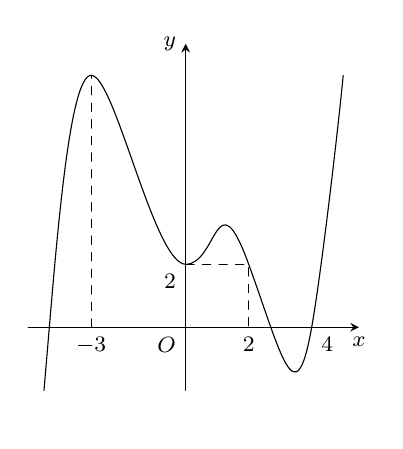
\begin{tikzpicture}[scale=0.4,font=\footnotesize,line join=round,line cap=round,>=stealth]%[x=.5cm,y=.5cm]
            \draw[-stealth] (-5,0)--(5.5,0)node[below]{$x$};
            \draw[-stealth] (0,-2)--(0,9) node[left]{$y$};
            \draw[dashed] (-3,0)node[below]{$-3$}--(-3,8) (0,2) node[below left]{$2$}-|(2,0)node[below]{$2$};
            \draw
            (-4.5,-2) .. controls +(85:4) and +(180:.75) .. (-3,8)
            .. controls +(0:.75) and +(180:1) .. (0,2)
            .. controls +(0:1) and +(110:3) .. (2,2)
            .. controls +(-70:3) and +(-100:3) .. (4,0)node[below right]{$4$}
            ..controls +(80:2) and +(-95:1) .. (5,8)
            (0,0) node[below left]{$O$}
            ;
        \end{tikzpicture}
    }
    \loigiai{
        Đặt $2x=t$ thì $t\in [-3;4]$ và ta đưa về xét $h(t)=f(t)-2t$.\\
        Ta có $h'(t)=f'(t)-2$ nên dựa vào đồ thị đã cho thì $h'(t)=0$ có hai nghiệm $t=0,t=2,$ trong đó $f'(t)-2$ lại không đổi dấu khi qua $t=0,$ còn $h'(t)$ đổi dấu từ $+$ sang $-$ khi qua $t=2$. \\
        Bảng biến thiên cho $h(t)$ trên $[-3;4]$ là
        \begin{center}
            \begin{tikzpicture}[scale=1]
                \tkzTabInit[ nocadre=false, lgt=1.3, espcl=2.5]{$t$ /1,$h'(t)$ /1,$h(t)$ /2}{$-3$,$0$,$2$,$4$}
                \tkzTabLine{,+,$0$,+,$0$,-,}
                \draw ($(N13)+(0,0.2)$)node[below](A){ } (N32)	node[below](B){$h(2)$} ($(N43)+(0,0.25)$)	node[below](C){ };
                \draw[-stealth] (A)--(B);
                \draw[-stealth] (B)--(C);
            \end{tikzpicture}
        \end{center}
        Dựa vào bảng biến thiên, ta có
        $\max\limits_{\left[-3;4\right]}h\left(t\right)=h(2)=f(2)-4=6$.
    }
\end{ex}
\Closesolutionfile{ans}